\section{Connessioni}
\subsection{NAS e SAN}
Per connettere attraverso la rete dei client ed uno storage è possibile inserire nella rete un \textit{Network Attached Storage (NAS)} che può fornire file direttamente ai client.

\begin{figure}[H]
    \centering
    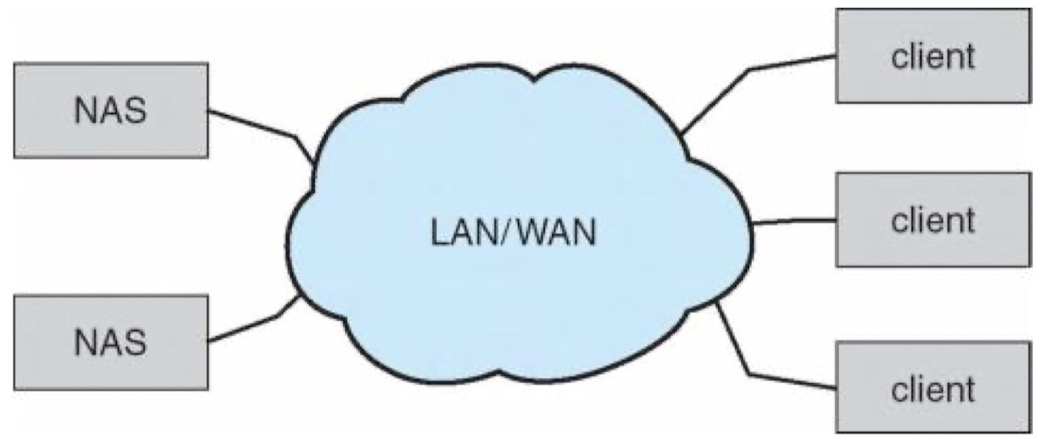
\includegraphics[width=0.5\linewidth]{assets/NAS-client.jpg}
\end{figure}

Oppure, con lo scopo di mantenere un livello di sicurezza più elevato, si possono inserire dei server tra i client e i NAS. In questo caso tra server e NAS si trova una rete privata, ovvero una \textit{Storage Area Network (SAN)}

\begin{figure}[H]
    \centering
    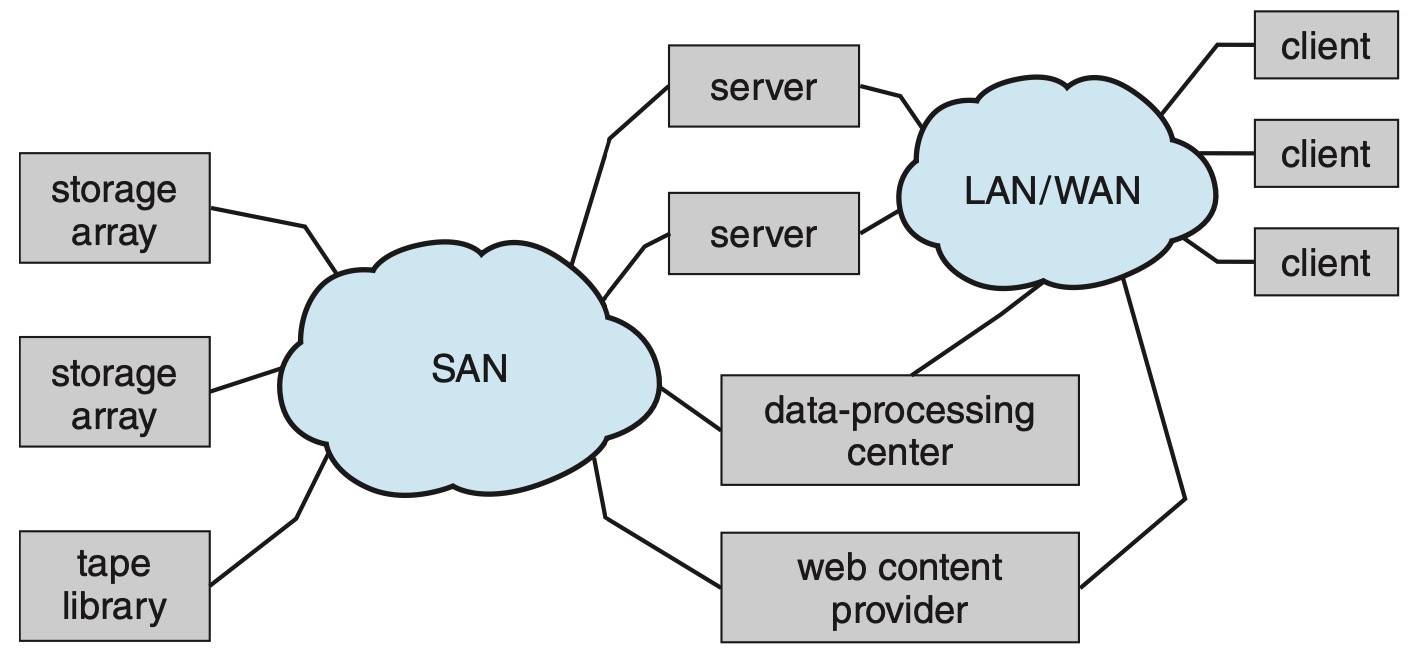
\includegraphics[width=0.5\linewidth]{assets/san.jpg}
\end{figure}

\subsection{SCSI}
Permette la connessione in parallelo di più dispositivi, fino a 16.

\subsection{Fiber Channel}
Architettura Seriale ad alta velocità, può gestire uno spazio di indirizzi a 24 bit ed è spesso alla base di SAN.